%%%%%%%%%%%%%%%%%%%%%%%%%%%%%%%%%%%%%%%%%%%%%%%%%%%%%%%%%%%%%%%%
%%%%%%%%%%%%%%%%%%%%%%%%%%%%%%%%%%%%%%%%%%%%%%%%%%%%%%%%%%%%%%%%
%%%%
%%%% This text file is part of the source of 
%%%% `Introduction to High-Performance Scientific Computing'
%%%% by Victor Eijkhout, copyright 2012/3/4/5
%%%%
%%%% This book is distributed under a Creative Commons Attribution 3.0
%%%% Unported (CC BY 3.0) license and made possible by funding from
%%%% The Saylor Foundation \url{http://www.saylor.org}.
%%%%
%%%%
%%%%%%%%%%%%%%%%%%%%%%%%%%%%%%%%%%%%%%%%%%%%%%%%%%%%%%%%%%%%%%%%
%%%%%%%%%%%%%%%%%%%%%%%%%%%%%%%%%%%%%%%%%%%%%%%%%%%%%%%%%%%%%%%%

\emph{Source code control}\index{source code control} systems, also
called \emph{revision control}\index{revision control
  systems|see{source code control}}  or
\emph{version control}\index{version control systems|see{source code control}}
systems, are
a way of storing software, where not only the current version is
stored, but also all previous versions. 
This is done by maintaining a \indexterm{repository} for all versions,
while one or more users work on a `checked out' copy of the latest
version. Those of the users that are developers can then commit their
changes to the repository. Other users then update their local copy.
The repository typically resides on a remote machine that is reliably
backup up.

There are various reasons for keeping your source in a repository.
\begin{itemize}
\item If you work in a team, it is the best way to synchronize your
  work with your colleagues. It is also a way to document what changes
  were made, by whom, and why.
\item It will allow you to roll back a defective code to a version
  that worked.
\item It allows you to have branches, for instance for customizations
  that need to be kept out of the main development line. If you are
  working in a team, a branch is a way to develop a major feature, stay up
  to date with changes your colleagues make, and only add your feature
  to the main development when it is sufficiently tested.
\item If you work alone, it is a way to synchronize between more than
  one machine. (You could even imagine traveling without all your
  files, and installing them from the repository onto a borrowed
  machine as the need arises.)
\item Having a source code repository is one way to backup your work.
\end{itemize}

There are various source code control systems; in this tutorial you
can learn the basics of \indexterm{Subversion} (also called
\emph{svn}), which is probably the most popular of the traditional
source code control systems, and Mercurial (or~\n{hg}), which is an
example of the new generation of \indextermsub{distributed}{source
code control} systems.

\Level 0 {Workflow in source code control systems}

Source code control systems are built around the notion
of \indexterm{repository}: a central store of the files of a project,
together with their whole history. Thus, a repository allows you to
share files with multiple people, but also to roll back changes, apply
patches to old version, et cetera.

The basic actions on a repository are:
\begin{itemize}
\item Creating the repository; this requires you to have space and
  write permissions on some server. Maybe your sysadmin has to do it
  for you.
\item Checking out the repository, that is, making a local copy of its
  contents in your own space.
\item\label{it:commit} Adding your changes to the repository, and
\item Updating your local copy with someone else's changes.
\end{itemize}
Adding your own changes is not always possible: there are many projects
where the developer allows you to check out the repository, but not to
incorporate changes. Such a repository is said to be read-only.

Figure~\ref{fig:svn} illustrates these actions for the Subversion system.
\begin{figure}[ht]
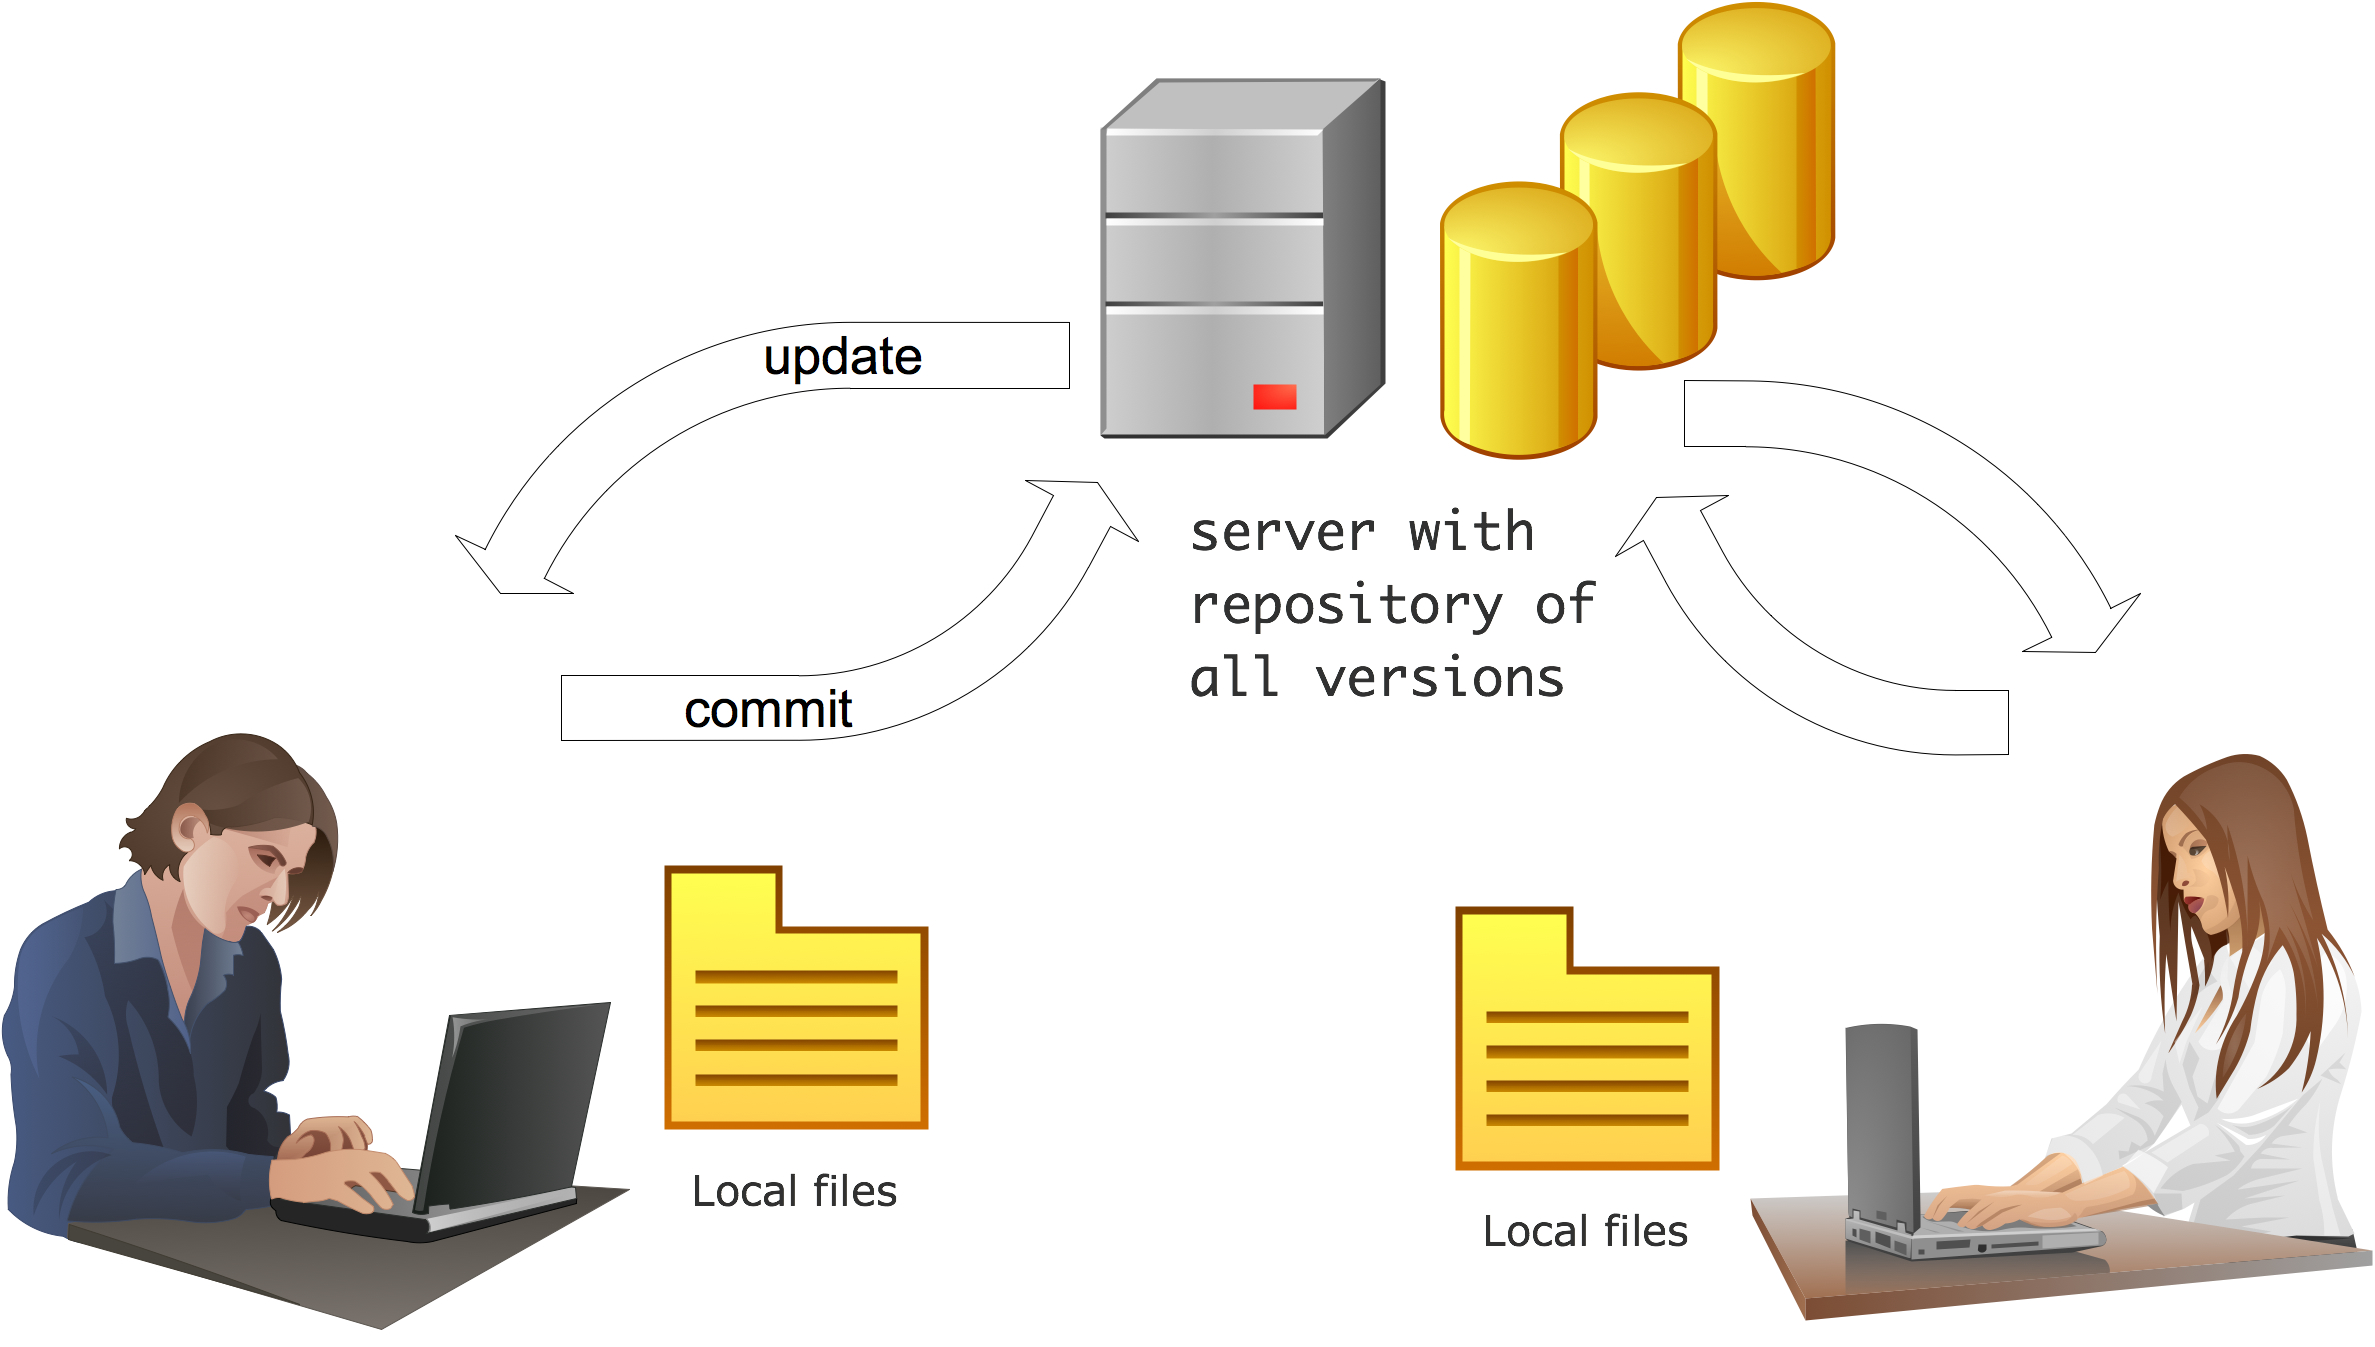
\includegraphics[scale=.17]{graphics/repo-flow-svn}
\caption{Workflow in traditional source code control systems such as Subversion}
\label{fig:svn}
\end{figure}
Users who have checked out the repository can edit files, and check in
the new versions with the \n{commit} command; to get the changes
committed by other users you use \n{update}.

One of the uses of committing is that you can roll your code back to
an earlier version if you realize you made a mistake or introduced a
bug. It also allows you to easily see the difference between different
code version. However, committing many small changes may be confusing
to other developers, for instance if they come to rely on something
you introduce which you later remove again. For this reason,
\indextermsub{distributed}{source code control} systems use two levels
of repositories.

There is still a top level that is authoritative, but
now there is a lower level, typically of local copies, where you can
commit your changes and accumulate them until you finally add them to
the central repository.
\begin{figure}[ht]
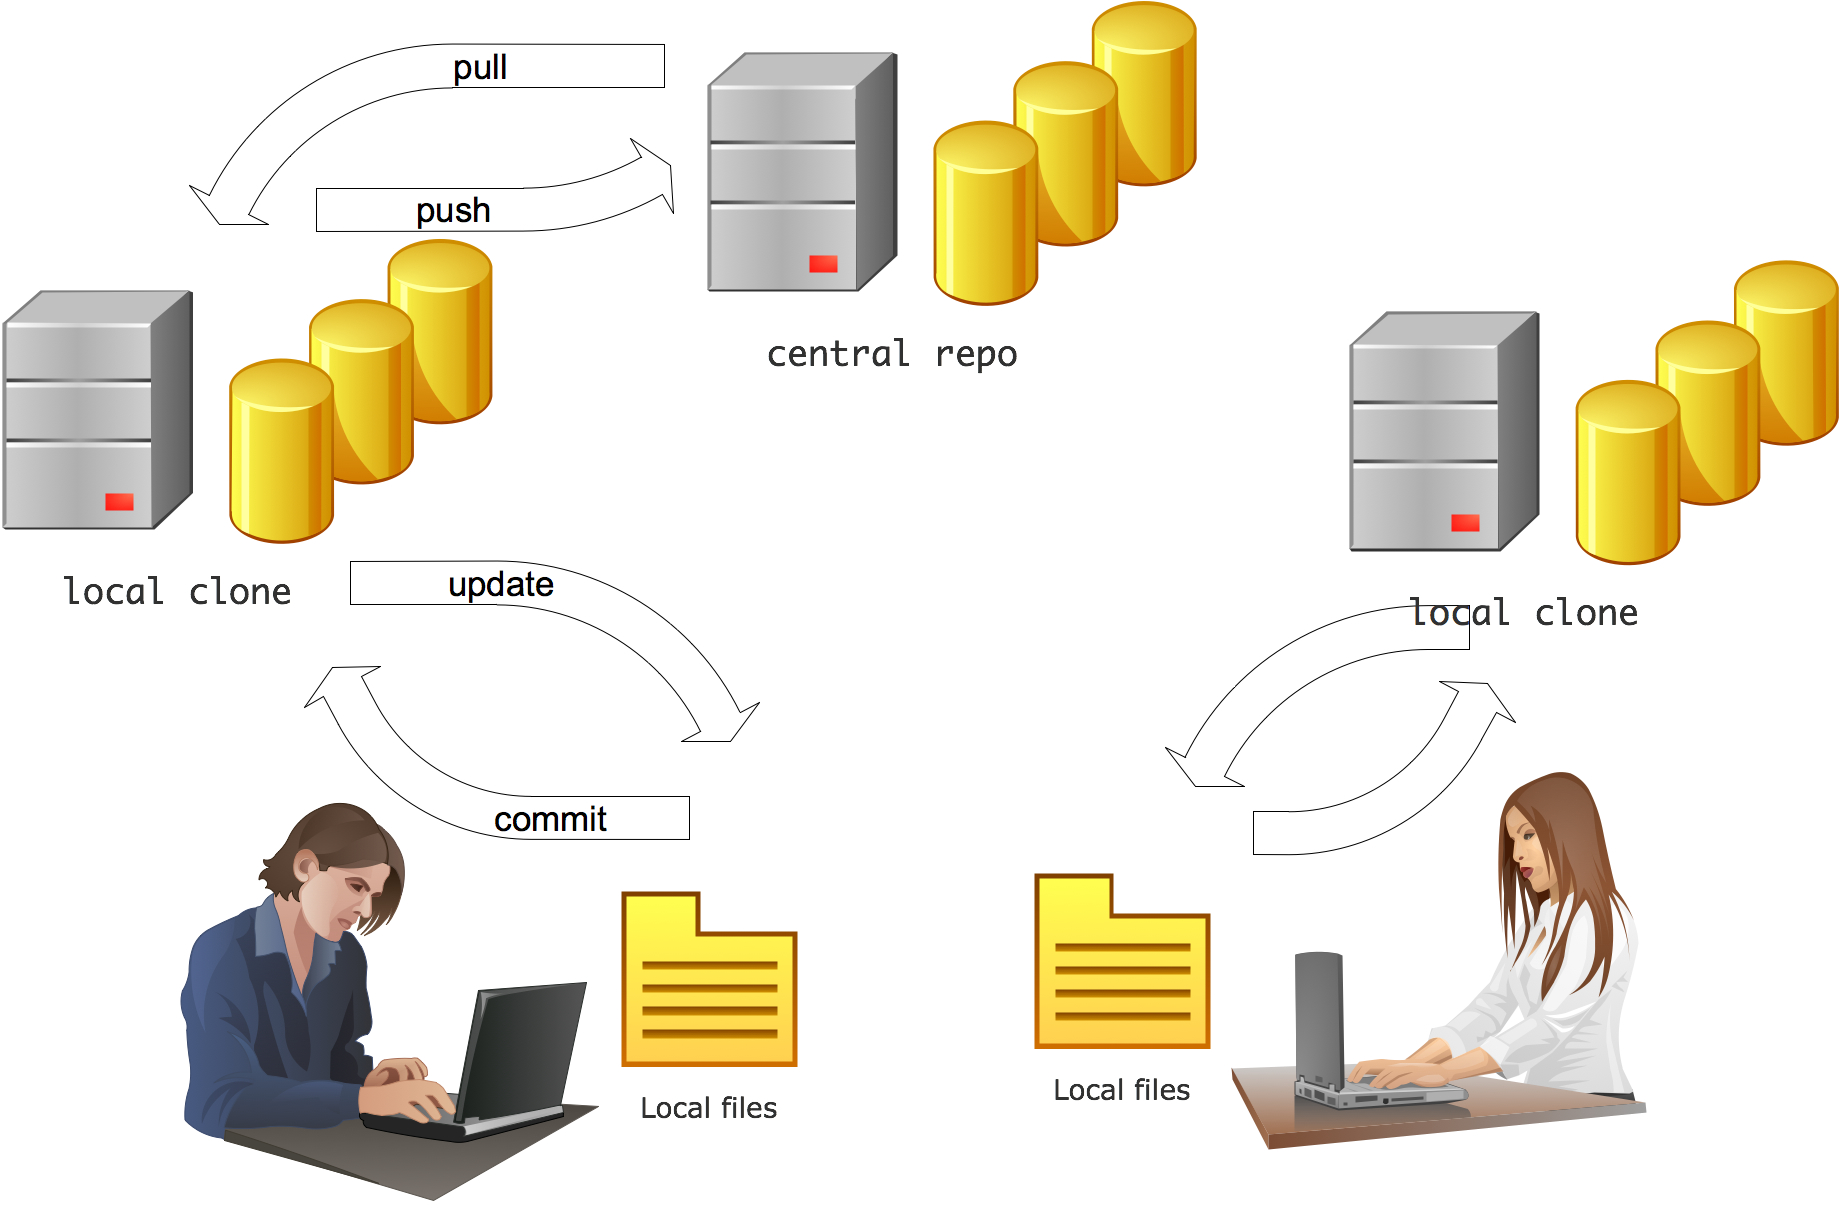
\includegraphics[scale=.19]{graphics/repo-flow-hg}
\caption{Workflow in distributed source code control systems such as Mercurial}
\label{fig:hg}
\end{figure}
This also makes it easier to contribute to a read-only repository:
you make your local changes, and when you are finished you tell the 
developer to inspect your changes and pull them into the top level 
repository. This structure is illustrated in figure~\ref{fig:hg}.

\Level 0 {Subversion or SVN}
\index{Subversion|(}
\index{svn|see{Subversion}}

This lab should be done two people, to simulate a group of programmers
working on a joint project. You can also do this on your own by using
two copies of the repository.

\Level 1 {Create and populate a repository}

\begin{purpose}
  In this section you will create a repository and make a local copy
  to work on.
\end{purpose}

First we need to have a repository. In practice, you will often use
one that has been set up by a sysadmin, but there are several ways to
set up a repository yourself.
\begin{itemize}
\item There are commercial and free hosting services such as 
  \indextermbus{Google}{code}
  \url{http://code.google.com/projecthosting} (open source only) or
  \indexterm{BitBucket} \url{https://bitbucket.org/}
  (this has favourable academic licenses). Once you create a
  repository there, you can make a local copy on your computer:
\begin{verbatim}
%% svn co http://yourservice.com//yourproject/ project
Checked out revision 0.
\end{verbatim}
where \n{co} is short for `check out'\footnote{Alternatively, you can create a repository in the local file system with \n{svnadmin create ./repository --fs-type=fsfs} and check it out with \n{svn co file://path.../}; we will not go into this.}.
\end{itemize}
You now have an empty directory \n{project}.

\practical{Go into the project directory and see if it is really
  empty.}{There is a hidden directory \n{.svn}}{}

The project directory knows where the master copy of the repository is
stored.

\practical{Do \n{svn info}}{You will see the URL of the repository
  and the revision number}{Make sure you are in the right
  directory. In the outer directories, you will get \n{svn: warning:
    '.' is not a working copy}}


\Level 1 {New files}

\begin{purpose}
  In this section you will make some simple changes: editing an
  existing file and creating a new file.
\end{purpose}

One student now makes a file to add to the repository\footnote{It is
  also possible to use \n{svn import} to create a whole repository
  from an existing directory tree.}.
\begin{verbatim}
%%  cat > firstfile
a
b
c
d
e
f
^D
\end{verbatim}
This file is unknown to \n{svn}:
\begin{verbatim}
%% svn status
?       firstfile
\end{verbatim}
We need to declare the file as belonging to the repository; a
subsequent \n{svn commit} command then copies it into the master repository.
\begin{verbatim}
%% svn add firstfile 
A         firstfile
%% svn status
A       firstfile
%% svn commit -m "made a first file"
Adding         firstfile
Transmitting file data .
Committed revision 1.
\end{verbatim}

\practical{The second student can now do \n{svn update} to update their
  copy of the repository}{\n{svn} should report \n{A  firstfile} and
  \n{Updated to revision 1.}. Check that the contents of the file are
  correct.}{In order to do the update command, you have to be in a
  checked-out copy of the repository. Do \n{svn info} to make sure
  that you are in the right place.}

\practical{Let both students create a new directory with a few
  files. Declare the directory and commit it. Do \n{svn update} to
  obtain the changes the other mde.}{You can do \n{svn add} on the
  directory, this will also add the files contained in it.}{Do not
  forget the \n{commit}.}

In order for svn to keep track of your files, you should never do
\n{cp} or \n{mv} on files that are in the repository. Instead, do
\n{svn cp} or \n{svn mv}. Likewise, there are commands \n{svn rm} and
\n{svn mkdir}.

\Level 1 {Conflicts}

\begin{purpose}
  In this section you will learn about how do deal with conflicting
  edits by two users of the same repository.
\end{purpose}

Now let's see what happens when two people edit the same file.
Let both students make an edit to \verb+firstfile+, but one to the
top, the other to the bottom. After one student commits the edit, the
other will see
\begin{verbatim}
%% emacs firstfile # make some change
%% svn commit -m "another edit to the first file"
Sending        firstfile
svn: Commit failed (details follow):
svn: Out of date: 'firstfile' in transaction '5-1'
\end{verbatim}
The solution is to get the other edit, and commit again. After the
update, svn reports that it has resolved a conflict successfully.
\begin{verbatim}
%% svn update
G  firstfile
Updated to revision 5.
%% svn commit -m "another edit to the first file"
Sending        firstfile
Transmitting file data .
Committed revision 6.
\end{verbatim}
The \n{G} at the start of the line indicates that svn has resolved a
conflicting edit.

If both students make edits on the same part of the file, svn can no
longer resolve the conflicts. For instance, let one student insert a
line between the first and the second, and let the second student edit
the second line. Whoever tries to commit second, will get messages
like this:
\begin{verbatim}
%% svn commit -m "another edit to the first file"
svn: Commit failed (details follow):
svn: Aborting commit: '/share/home/12345/yourname/myproject/firstfile' 
remains in conflict
%% svn update
C  firstfile
Updated to revision 7.
\end{verbatim}
Subversion will give you several options. For instance, you can type
\n{e} to open the file in an editor. You can also type \n{p} for
`postpone' and edit it later.
Opening the file in an editor, it will look like
\begin{verbatim}
aa
<<<<<<< .mine
bb
=======
123
b
>>>>>>> .r7
cc
\end{verbatim}
indicating the difference between the local version (`mine') and the
remote. You need to edit the file to resolve the conflict.

After this, you tell svn that the conflict was resolved, and
you can commit:
\begin{verbatim}
%% svn resolved firstfile
Resolved conflicted state of 'firstfile'
%% svn commit -m "another edit to the first file"
Sending        firstfile
Transmitting file data .
Committed revision 8.
\end{verbatim}
The other student then needs to do another update to get the
correction.

\Level 1 {Inspecting the history}

\begin{purpose}
  In this section, you will learn how to get information about the repository.
\end{purpose}

You've already seen \n{svn info} as a way of getting information
about the repository. To get the history, do \n{svn log} to get all
log messages, or \n{svn log 2:5} to get a range.

To see differences in various revisions of individual files, use
\n{svn diff}. First do \n{svn commit} and \n{svn update} to
make sure you are up to date. Now do \n{svn diff firstfile}. No
output, right? Now make an edit in \n{firstfile} and do \n{svn diff
  firstfile} again. This gives you the difference between the last
commited version and the working copy.

You can also ask for differences between committed versions with
\n{svn diff -r 4:6 firstfile}.

The output of this diff command is a bit cryptic, but you can
understand it without too much trouble. There are also fancy GUI
implementations of svn for every platform that show you differences in
a much nicer way.

If you simply want to see what a file used to look like, do \n{svn
  cat -r 2 firstfile}. To get a copy of a certain revision of the
repository, do \n{svn export -r 3 . ../rev3}, which exports the
repository at the current directory (`dot') to the directory \n{../rev3}.

If you save the output of \n{svn diff}, it is possible to apply it
with the Unix \n{patch} command. This is a quick way to send patches
to someone without them needing to check out the repository.

\Level 1 {Shuffling files around}

We now realize that we really wanted all these files in a subdirectory
in the repository. First we create the directory, putting it under svn control:
\begin{verbatim}
%% svn mkdir trunk
A         trunk
\end{verbatim}
Then we move all files there, again prefixing all comands with \n{svn}:
\begin{verbatim}
%% for f in firstfile otherfile myfile mysecondfile ; do \
        svn mv $f trunk/ ; done
A         trunk/firstfile
D         firstfile
A         trunk/otherfile
D         otherfile
A         trunk/myfile
D         myfile
A         trunk/mysecondfile
D         mysecondfile
\end{verbatim}
Finally, we commit these changes:
\begin{verbatim}
%% svn commit -m "trunk created"
Deleting       firstfile
Adding         trunk/firstfile
Deleting       myfile
Deleting       mysecondfile
Deleting       otherfile
Adding         trunk
Adding         trunk/myfile
Adding         trunk/mysecondfile
Adding         trunk/otherfile
\end{verbatim}

You probably now have picked up on the message that you always use
\n{svn} to do file manipulations. Let's pretend this has slipped your
mind.

\practical{Create a file \n{somefile} and commit it to the repository.
Then do \n{rm somefile}, thereby deleting a file without
  \n{svn} knowing about it.
What is the output of \n{svn status}?}{svn indicates with an
  exclamation point that the file has disappeared.}{}

You can fix this situation in a number of ways:
\begin{itemize}
\item \n{svn revert} restores the file to the state in which it was
  last restored. For a deleted file, this means that it is brought
  back into existence from the repository. This command is also useful to
  undo any local edits, if you change your mind about something.
\item \n{svn rm firstfile} is the official way to delete a file. You
  can do this even if you have already deleted the file outside
  \n{svn}.
\item Sometimes \n{svn} will get confused about your attempts to
  delete a file. You can then do \n{svn --force rm yourfile}.
\end{itemize}

\Level 1 {Branching and merging}

Suppose you want to tinker with the repository, while still staying up
to date with changes that other people make.
\begin{verbatim}
%% svn copy \
  <the URL of your repository>/trunk \
  <the URL of your repository>/onebranch \
  -m "create a branch"

Committed revision 11.
\end{verbatim}
You can check this out as before:
\begin{verbatim}
%% svn co <the URL of your repository>/onebranch \
          projectbranch       
A  projectbranch/mysecondfile
A  projectbranch/otherfile
A  projectbranch/myfile
A  projectbranch/firstfile
Checked out revision 11.
\end{verbatim}

Now, if you make edits in this branch, they will not be visible in the
trunk:
\begin{verbatim}
%% emacs firstfile # do some edits here
%% svn commit -m "a change in the branch"
Sending        firstfile
Transmitting file data .
Committed revision 13.
%% (cd ../myproject/trunk/ ; svn update )
At revision 13.
\end{verbatim}

On the other hand, edits in the main trunk can be pulled into this
branch:
\begin{verbatim}
%% svn merge ^/trunk
--- Merging r13 through r15 into '.':
U    secondfile
\end{verbatim}
When you are done editing, the branch edits can be added back to the
trunk. For this, it is best to have a clean checkout of the branch:
\begin{verbatim}
%% svn co  file://`pwd`/repository/trunk mycleanproject
A    # all the current files
\end{verbatim}
and then do a special merge:
\begin{verbatim}
%% cd mycleanproject
%% svn merge --reintegrate ^/branch
--- Merging differences between repository URLs into '.':
U    firstfile
 U   .
%% svn info
Path: .
URL: <the URL of your repository>/trunk
Repository Root: <the URL of your repository>
Repository UUID: dc38b821-b9c6-4a1a-a194-a894fba1d7e7
Revision: 16
Node Kind: directory
Schedule: normal
Last Changed Author: build
Last Changed Rev: 14
Last Changed Date: 2009-05-18 13:34:55 -0500 (Mon, 18 May 2009)
%% svn commit -m "trunk updates from the branch"
Sending        .
Sending        firstfile
Transmitting file data .
Committed revision 17.
\end{verbatim}

\Level 1 {Repository browsers}

The \n{svn} command can give you some amount of information about a
repository, but there are graphical tools that are easier to use and
that give a better overview of a repository. For the common platforms,
several such tools exist, free or commercial. Here is a browser based
tool:~\url{http://wwww.websvn.info}.

\index{Subversion|)}

\input tutorials/mercurial
\endinput

\Level 0 {Other source control systems}

Lately, there has been considerable interest in `distributed source
code control' system, such as \indexterm{git} or
\indexterm{mercurial}. In these systems, each user has a local
repository against which commits can be made. This has some advantages
over systems like \n{svn}.

Consider the case where a developer is working on a  patch that takes some
time to code and test. During this time, development on the project
goes on, and by the time the patch can be commited, too many changes
have been made for \n{svn} to be able to merge the patch. As a result,
branching and merging is often a frustrating experience with
traditional system. In distributed systems, the developer can do
commits against the local repository, and roll back versions as
needed. Additionally, when the patch is ready to merge back, it is not
a single massive change, but a sequence of small changes, which the
source control system should be better able to handle.

